We tested the algorithms with three Monte Carlo simulations: a
geometry-only toy simulation to observe the geometric effects
independent of detector effects, a full Pythia and GEANT-based
$pp \to \mu + X$ collisions sample, and a full GEANT-based cosmic ray
sample.  The sizes of the simulated event samples are all large enough
for the alignment results to be systematics-limited, and in the
GEANT-based simulations, all detector effects were modelled except
tracker misalignment, magnetic field errors, and internal muon chamber
misalignment.  This demonstrates the alignment reach of the algorithms
themselves, apart from any possible deficiencies in the input
tracks, propagation model, and chamber geometry.

The initial muon system misalignment used in these studies was a
Gaussian smearing of chamber positions with a 2~mm standard deviation in $\delta_x$,
4~mm in $\delta_y$ and $\delta_z$, and 2~mrad in the three angles.  We
then applied each procedure to the simulated events in exactly the
same way we do to data.  Different initial misalignments yield the
same results.

Figure~\ref{fig:hip_MC} shows differences between aligned positions of
each parameter and their true positions for the two algorithms in
simulated cosmic rays.  Interpreting the RMS of these distributions as
the alignment accuracy, the $\delta_x$ accuracy is 200~$\mu$m for HIP,
500~$\mu$m for Millepede, close to the intrinsic hit uncertainty of
100--300~$\mu$m.  Statistical uncertainties returned by the fits are a
factor of 3--4 times smaller than the observed accuracy, so this
represents the systematic limit of the algorithms as they are
currently defined.

\begin{figure}
\subfigure[HIP aligned-minus-true positions before (purple) and after (yellow) alignment.]{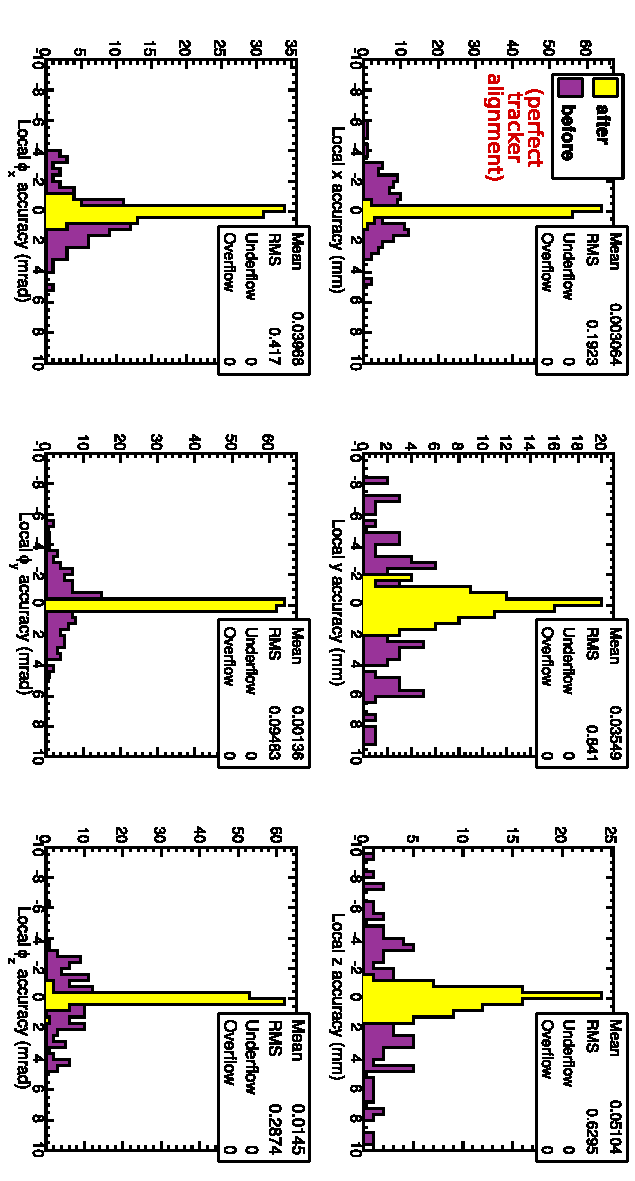
\includegraphics[height=\linewidth, angle=90]{plots/mc_and_syst_studies/hip_MC.pdf}}

\subfigure[Millepede aligned-minus-true positions before (purple) and after (yellow) alignment.]{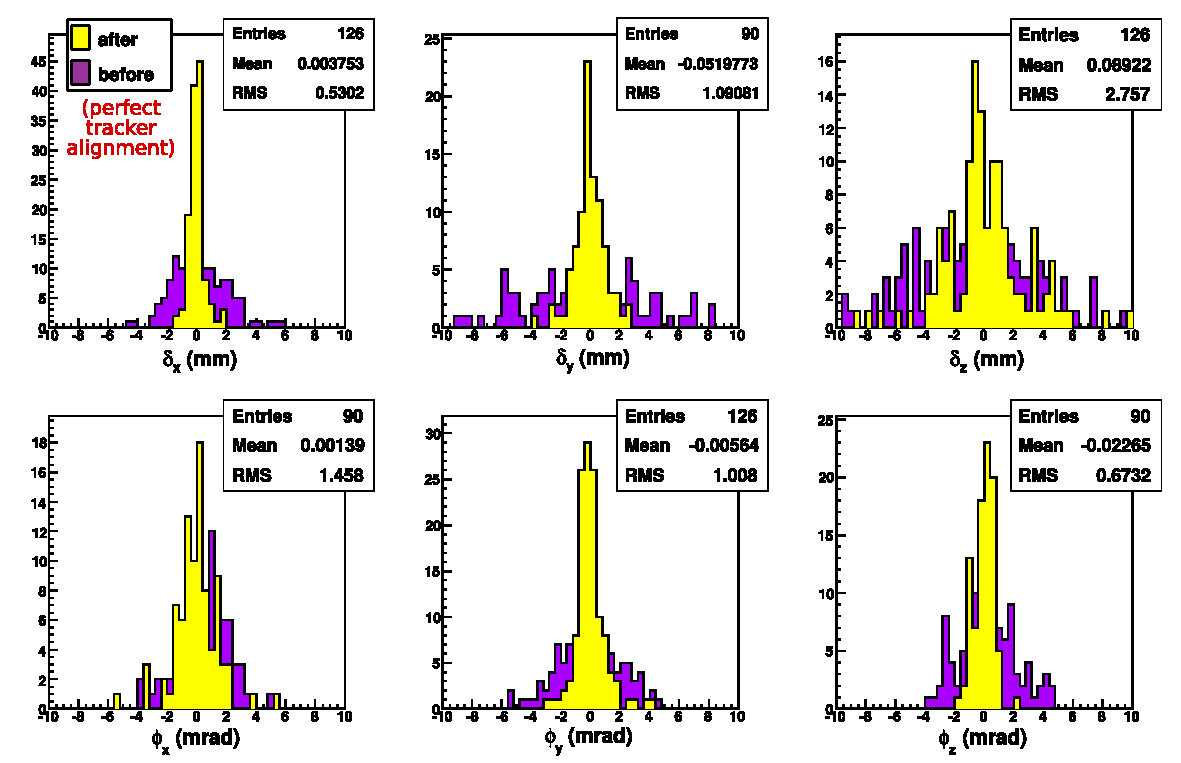
\includegraphics[width=\linewidth]{plots/mc_and_syst_studies/Millipede_MC_RandomScenario.pdf}}

\caption{Alignment with simulated cosmic rays using (a) HIP and (b) Millepede.  Each
  entry in the histograms is the difference between the aligned and
  true values of alignment parameters for one DT
  chamber.  (Only aligned parameters are shown: $\delta_x$,
  $\delta_{\phi_y}$ and $\delta_{\phi_z}$ for station~4 and all 6
  parameters for stations 1--3.) \label{fig:hip_MC}}
\end{figure}

There are four classes of systematic error in these procedures:
(1) simplifying assumptions about the residuals distributions,
(2) biases in the input set of tracks,
(3) errors in the propagation of tracks through the muon system, and
(4) internal misalignments in the chambers.
The exercise described above addresses the first of these, in that the
Monte Carlo simulation represents a complete model of the detector
response~\cite{ref:dtlocalreco}, while the alignment algorithms both
include simplifications, optimized for finding the underlying
misalignment.  The Millepede performance is expected to improve by
including a more realistic description of the covariance
${\sigma_{\mbox{\scriptsize resid}_{\mbox{\scriptsize
$i$}}}}^2$ (Equation~\ref{eqn:globalmpchi2}) and a better
treatment of the tails of the residuals distribution.

The question of whether input tracks were biased (2) can be addressed in several ways.
One is to compare local alignment information with global information,
as only the latter would be affected by a biased global tracks.  This
cross-check was performed and is presented in the next section.
Another test uses the fact that muon chambers are large rigid bodies:
residuals inside the chambers must be linear with respect to $x$, $y$,
$\tfrac{dx}{dz}$, and $\tfrac{dy}{dz}$, but can be discontinuous at
the thresholds between chambers.  Discontinuities such as these can
only be caused by misalignments, as the input track distribution is
unlikely to have features at these points.  Small input track biases, below
the limit of what could be observed by these methods, would distort
the aligned positions of chambers, but in such a way that optimizes
the tracking resolution of the selected input tracks.

As tracks propagate into the muon system (3), they may be systematically
distorted by potential errors in the magnetic field map and material
budget, in a way which reverses sign with muon charge.  Application of
the procedure described in~\ref{sec:hipalgo} to correct for this
effect resulted in negligible alignment differences (100~$\mu$m,
200~$\mu$m, and 350~$\mu$m
in $\delta_x$, $\delta_y$, and $\delta_z$ and 0.1~mrad in the angles).

Finally, internal misalignments (4) change the effective center of the
chamber, making the global alignment results harder to interpret in
comparison with physical landmarks (such as the hardware alignment
system), but no less valid for track reconstruction.

